\subsubsection{2.4. Đồ thị đa phương thức (MG)}
\indent\indent Đồ thị đa phương thức (MG) \cite{peng2024learningmultimodalgraphssurvey} là một cấu trúc dữ liệu cho phép mô hình hóa sự kết hợp giữa dữ liệu hình ảnh, văn bản và âm thanh trong một không gian thống nhất.\vspace{0.3cm}

Về mặt định nghĩa, một đồ thị đa phương thức $G = (V, E)$ được đặc trưng bởi hai thành phần:
\vspace{-0.1cm}
\begin{itemize}[label={--}, itemsep=1pt]
    \item Tập hợp các đỉnh $V$ chứa dữ liệu hoặc đặc trưng thuộc về một hoặc nhiều phương thức khác nhau.
    \item Tập hợp các cạnh $E$ thể hiện mối quan hệ tương tác giữa các đỉnh trong tập $V$.
\end{itemize}

\begin{figure}[H]
    \centering
    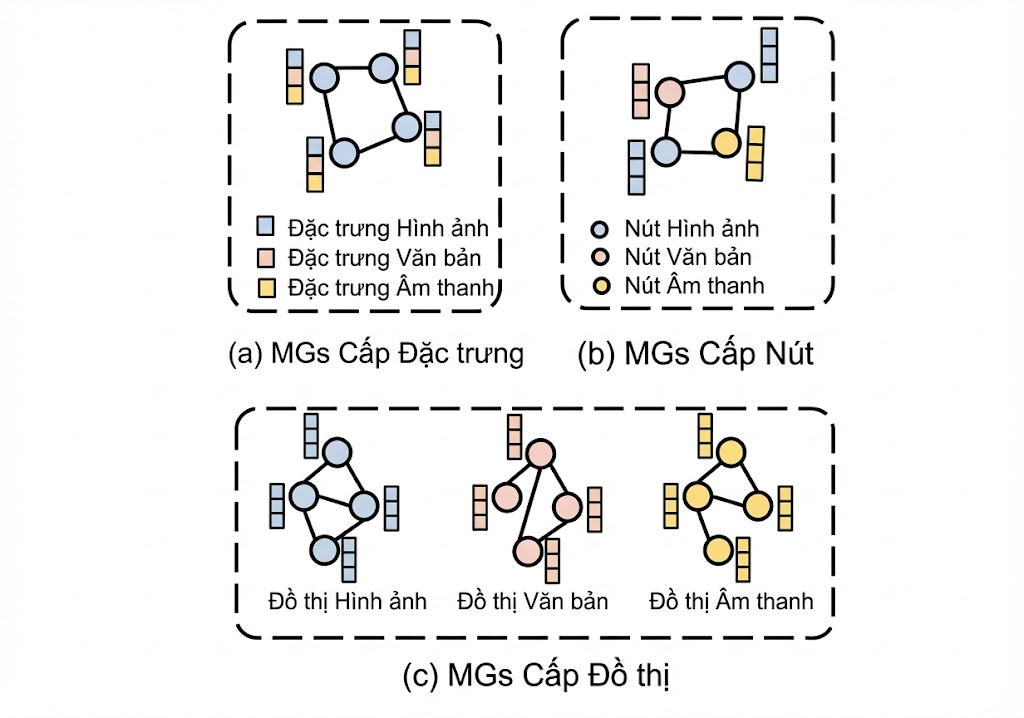
\includegraphics[width=0.8\linewidth]{images/part-02/chap-01/MG_ver2.jpg}
    \vspace{0.5cm}
    \caption{Các kiến trúc đồ thị đa phương thức phổ biến}
    \label{fig:MG}
\end{figure}

Dựa vào cách thức phân phối dữ liệu đa phương thức trên các đỉnh, cũng như cách mà chúng kết nối với nhau, Peng và cộng sự \cite{peng2024learningmultimodalgraphssurvey} đã tiến hành phân loại MG thành ba dạng kiến trúc chính:\vspace{-0.1cm}
\begin{itemize}[label={--}, itemsep=1pt]
    \item Đồ thị đa phương thức cấp đặc trưng (Feature-Level MG): Tại cấp độ này, tính đa phương thức được tích hợp ngay bên trong mỗi đỉnh của đồ thị. Mỗi đỉnh $v_i \in V$ lưu trữ một tập hợp các đặc trưng từ tất cả các phương thức có sẵn.
    \item Đồ thị đa phương thức cấp đỉnh (Node-Level MG): Trong kiến trúc này, mỗi đỉnh chỉ mang đặc trưng của một phương thức duy nhất (đơn phương thức), nhưng toàn bộ đồ thị là tập hợp của các đỉnh thuộc nhiều loại phương thức khác nhau cùng tồn tại và kết nối.
    \item Đồ thị đa phương thức cấp đồ thị (Graph-Level MG): Loại đồ thị này được xây dựng từ một tập các đồ thị con (subgraphs), trong đó mỗi đồ thị con mô tả cấu trúc quan hệ của các thực thể dưới góc nhìn của một phương thức riêng biệt. Đặc biệt, các cạnh chỉ tồn tại giữa các đỉnh thuộc cùng một đồ thị con, tức là các kết nối chỉ được thiết lập trong phạm vi từng phương thức và không có kết nối trực tiếp giữa các đỉnh thuộc các phương thức khác nhau.
\end{itemize}